\chapter{Embedded Hardware}

\noindent This appendix shows the complete embedded system hardware design, including the 3D model, copper layer layouts, and schematic pages for the hydrogel 3D printer control circuit.

\section{PCB Layout}
\begin{center}
  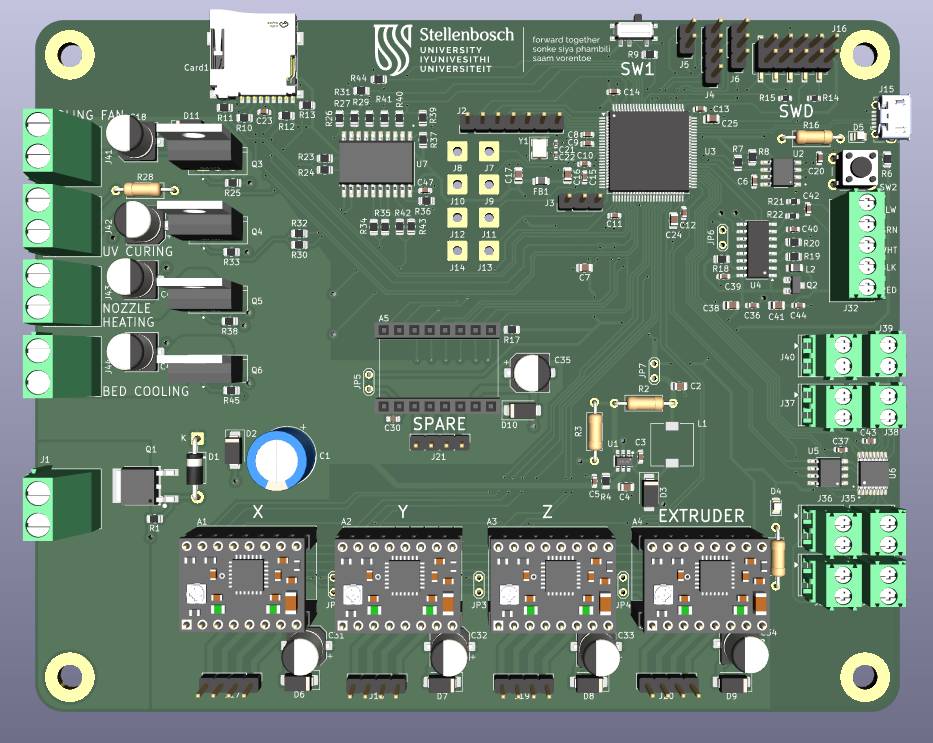
\includegraphics[width=0.62\textheight]{chaps-append/PCB_3D_view.png}
  \captionof{figure}{3D model of the assembled PCB illustrating overall component layout}
  \label{fig:pcb_3d_view}

  \vspace{1em}
  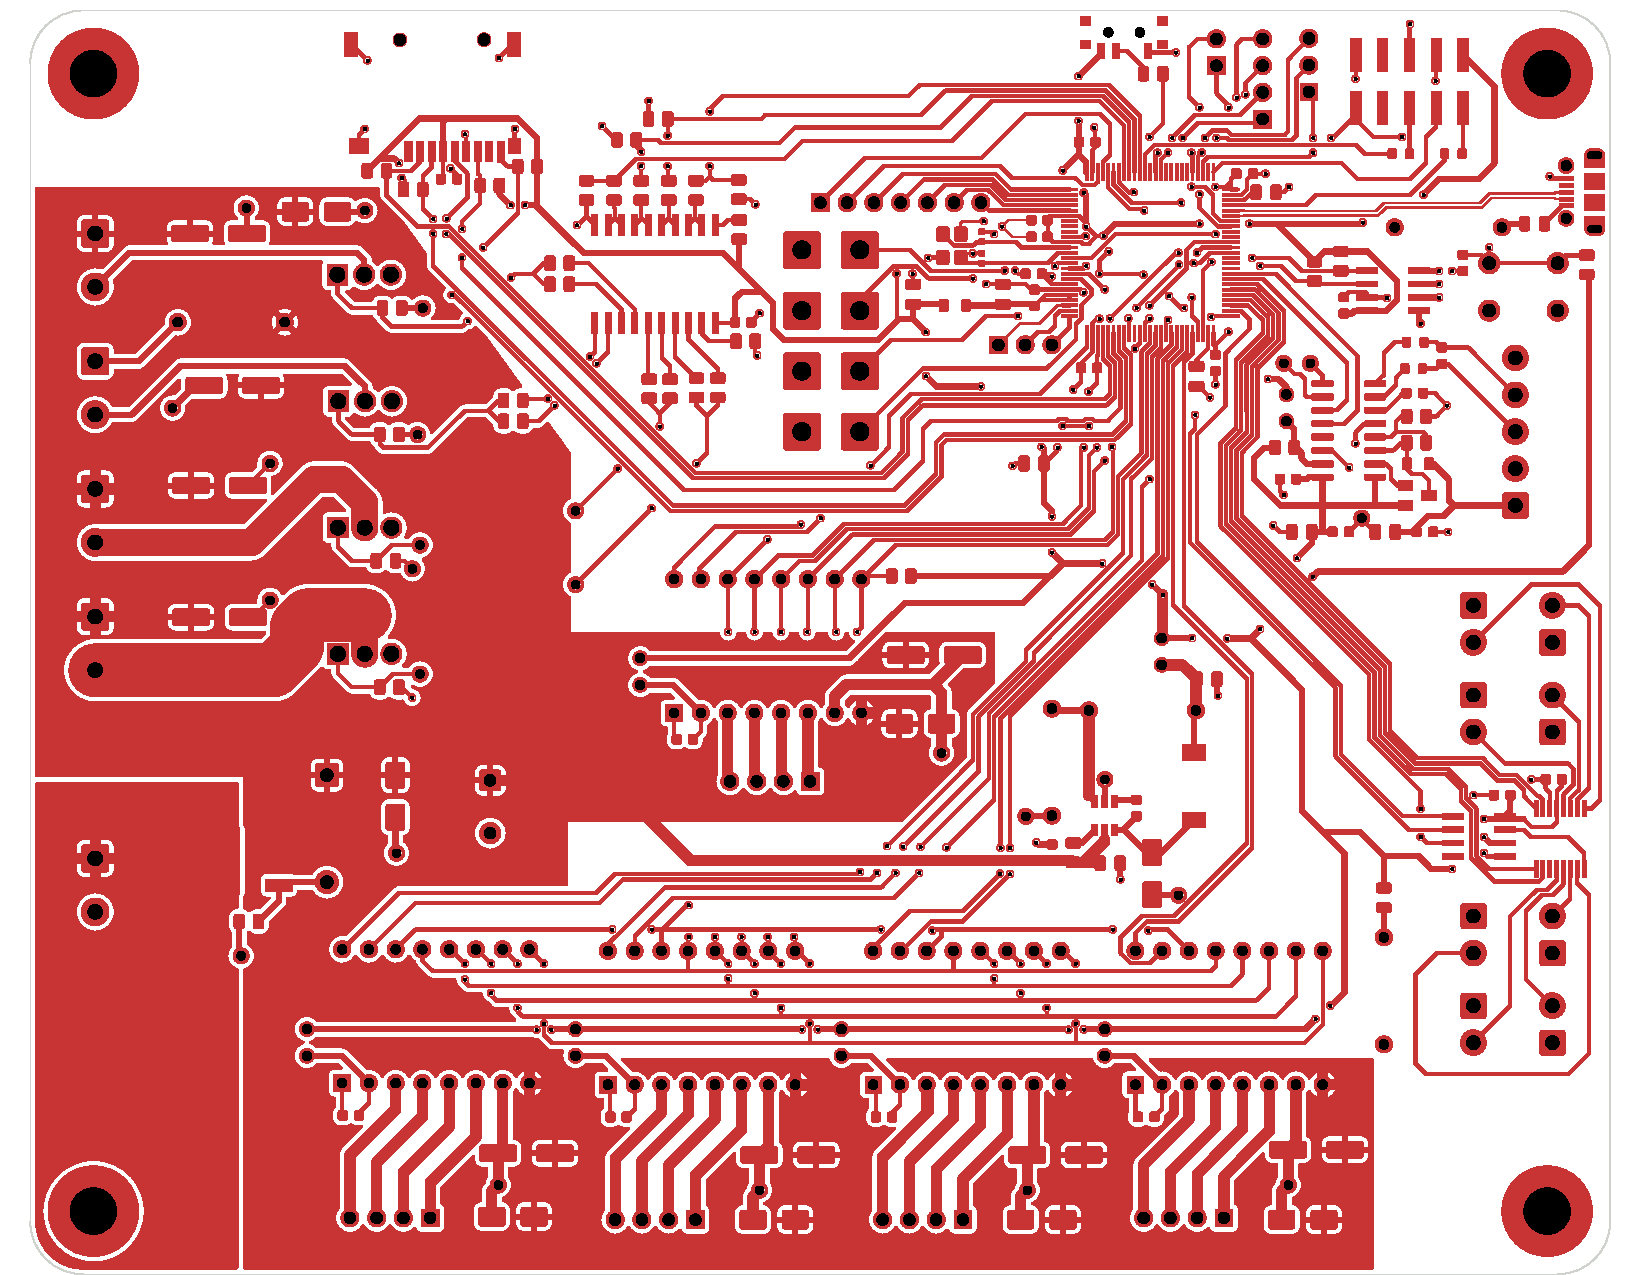
\includegraphics[width=0.56\textheight]{chaps-append/PCB_top_layer.pdf}
  \captionof{figure}{Top layer layout showing signal routing and power traces.}
  \label{fig:pcb_top_layer}

  \vspace{1em}
  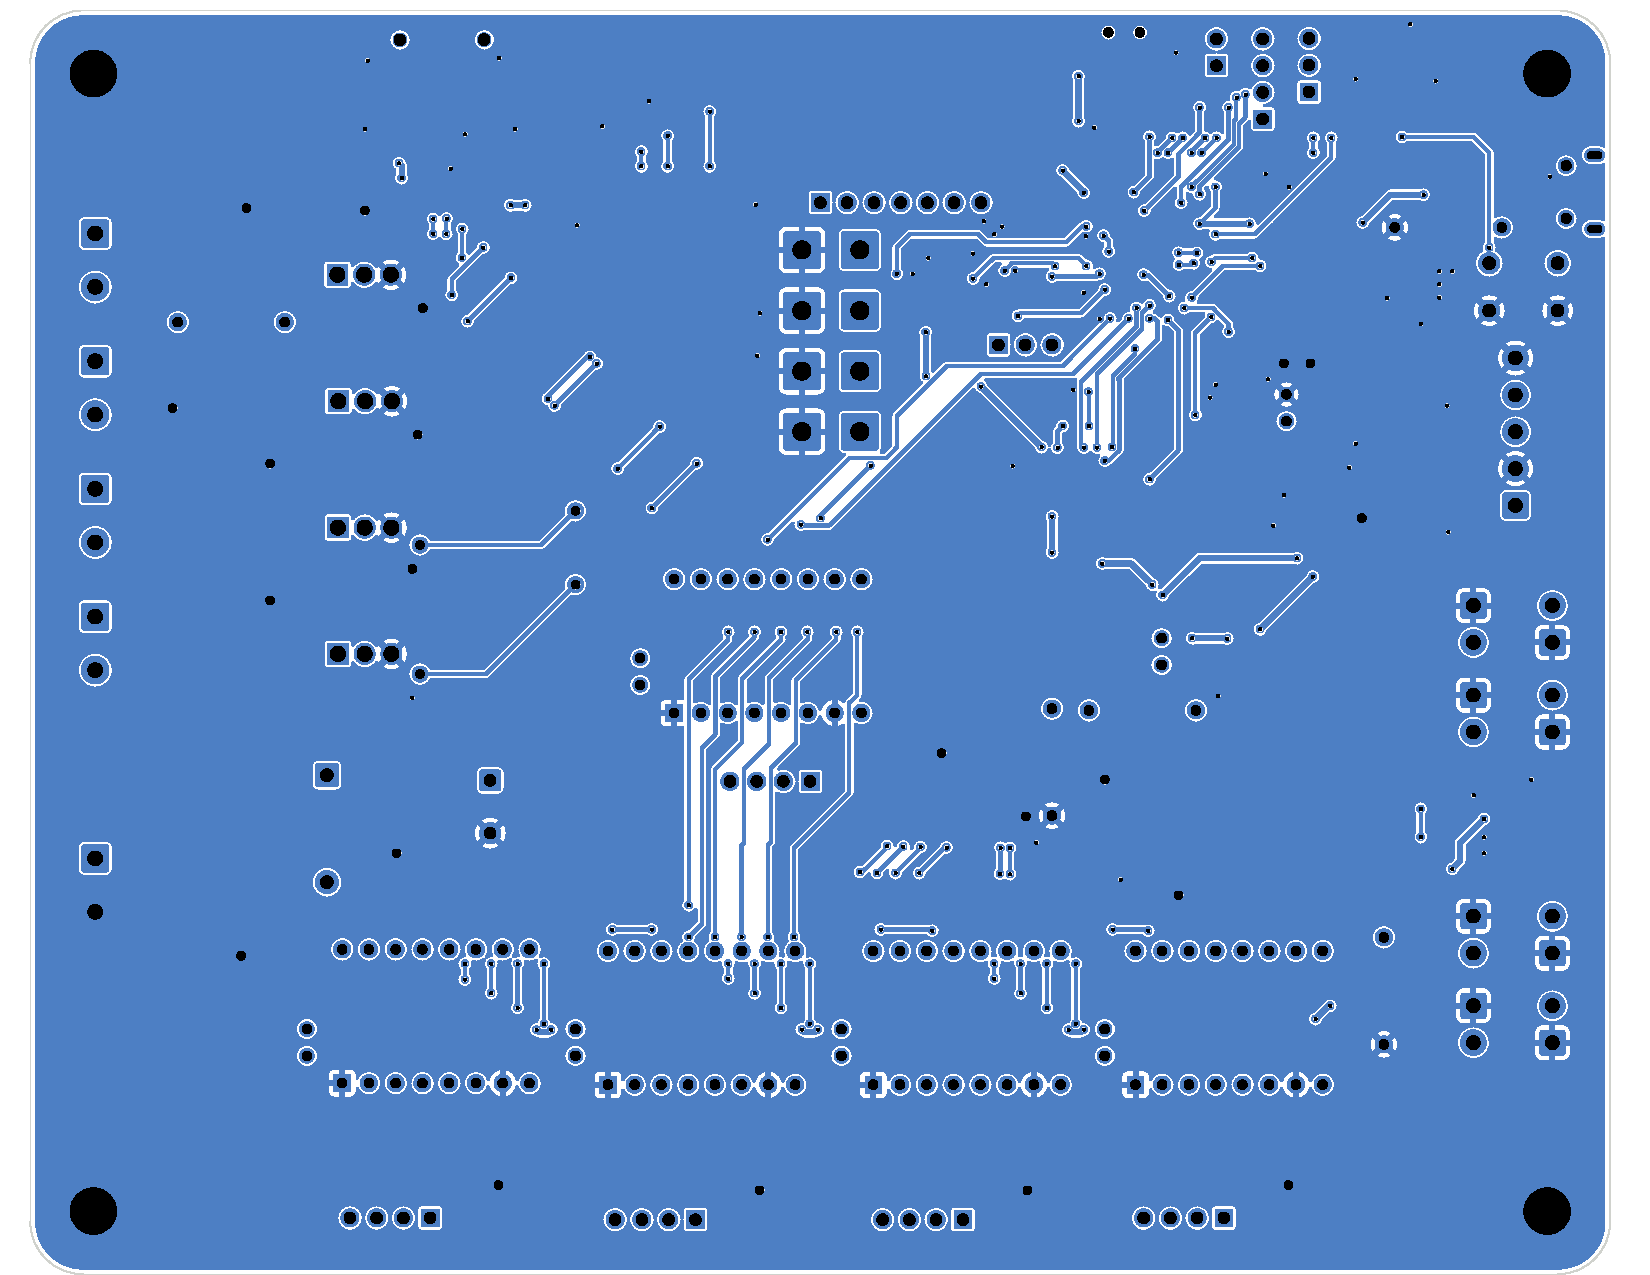
\includegraphics[width=0.56\textheight]{chaps-append/PCB_bottom_layer.pdf}
  \captionof{figure}{Bottom layer layout showing ground planes, vias, and routing.}
  \label{fig:pcb_bottom_layer}
\end{center}

\section{Circuit Schematics}
\begin{center}
  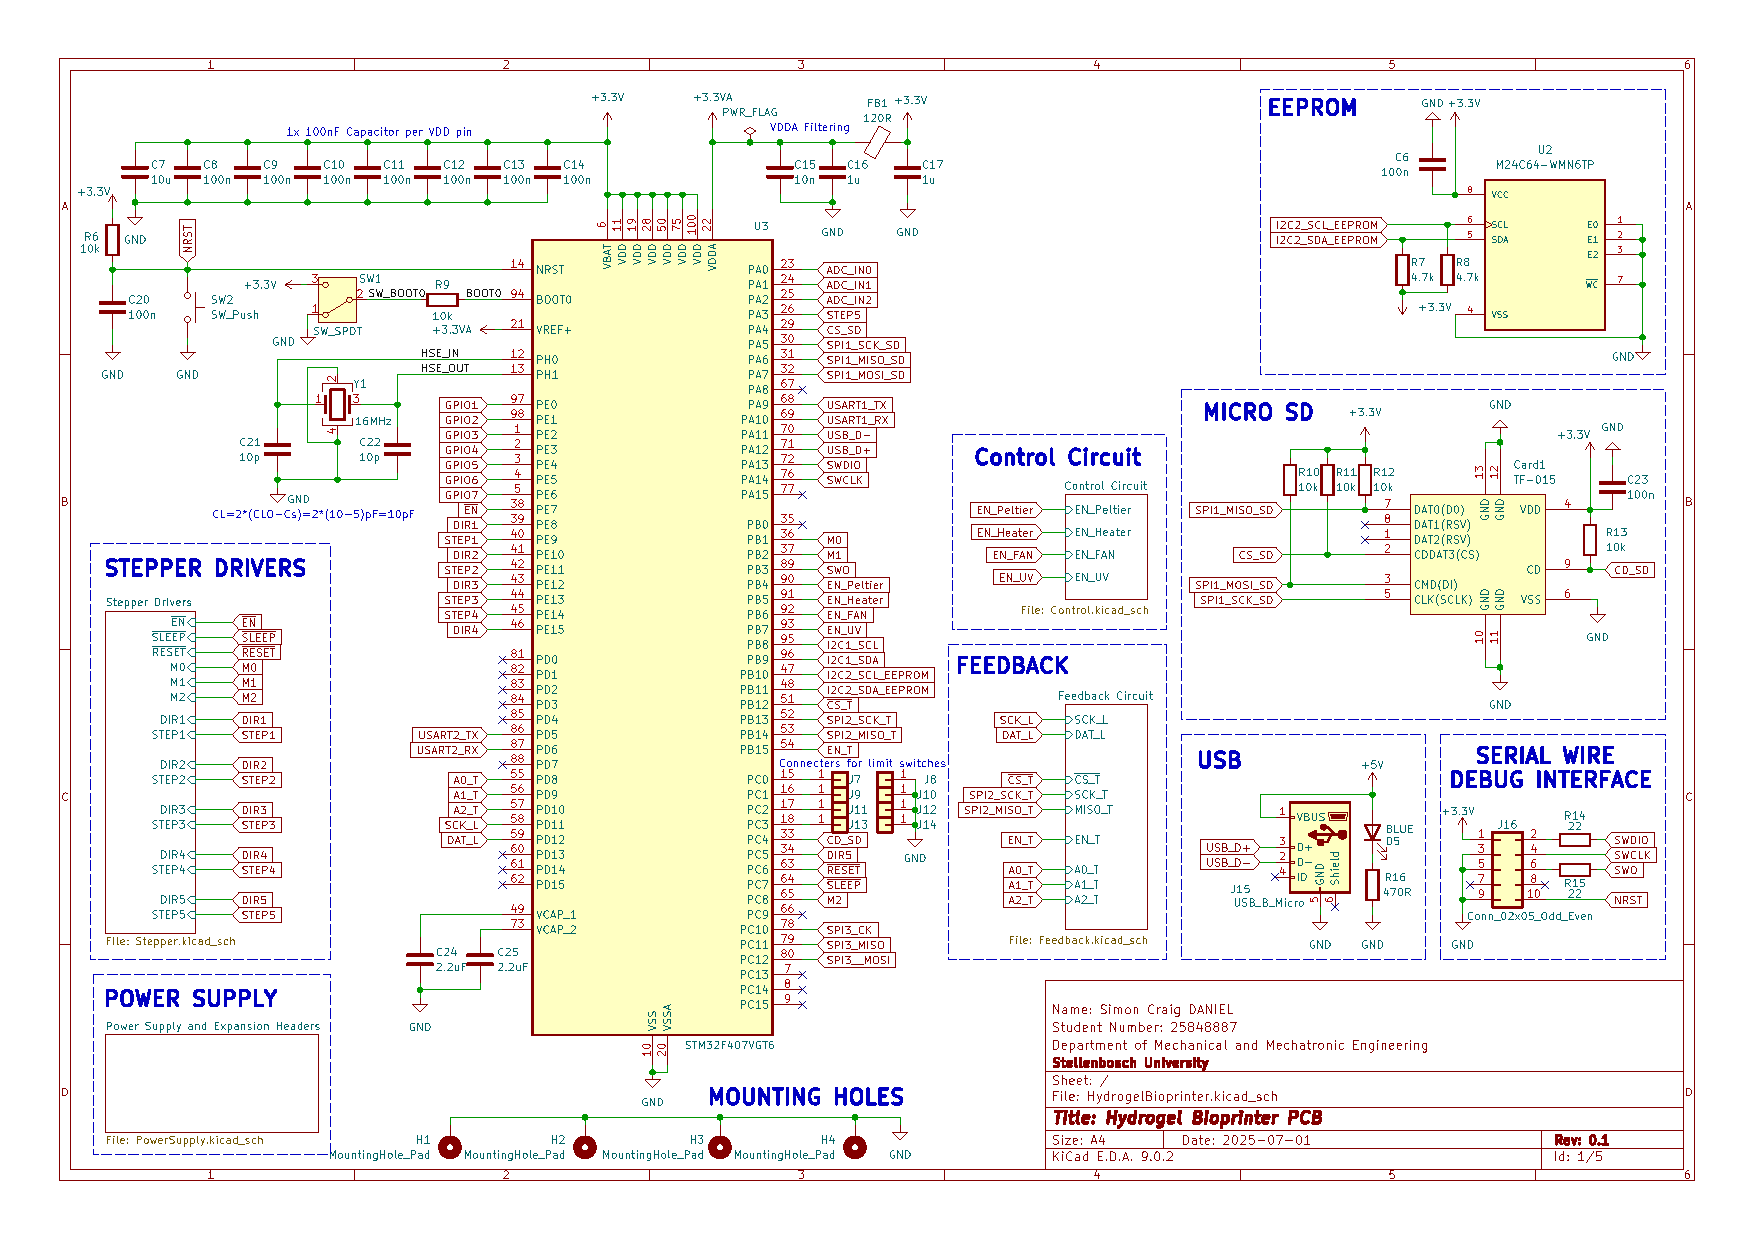
\includegraphics[angle=90, width=0.64\textheight]{chaps-append/PCBSchematic_Page1.pdf}
  \captionof{figure}{Schematic overview of the bioprinter control board.}
  \label{fig:pcb_overview}

  \vspace{1em}
  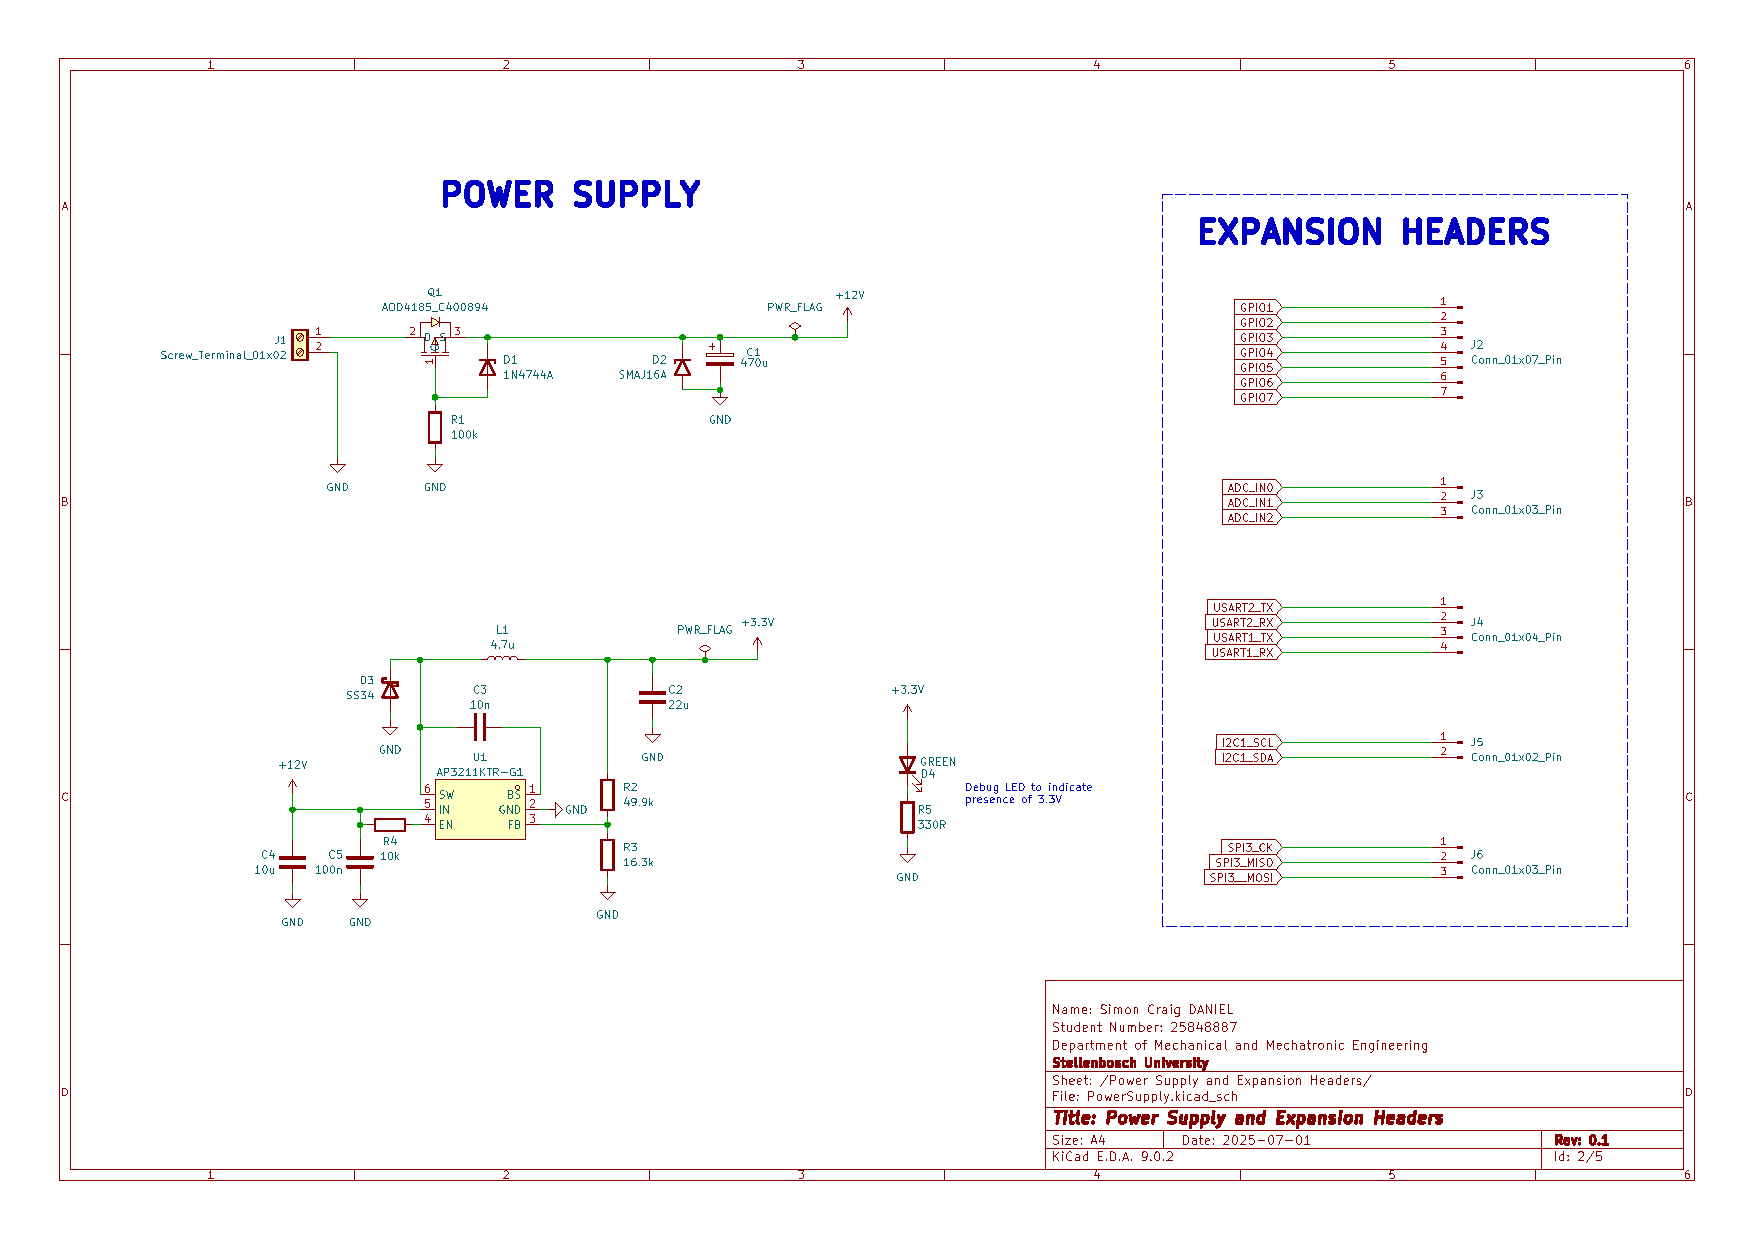
\includegraphics[angle=90, width=0.64\textheight]{chaps-append/PCBSchematic_Page2.pdf}
  \captionof{figure}{Bioprinter power supply system schematic.}
  \label{fig:pcb_power}

  \vspace{1em}
  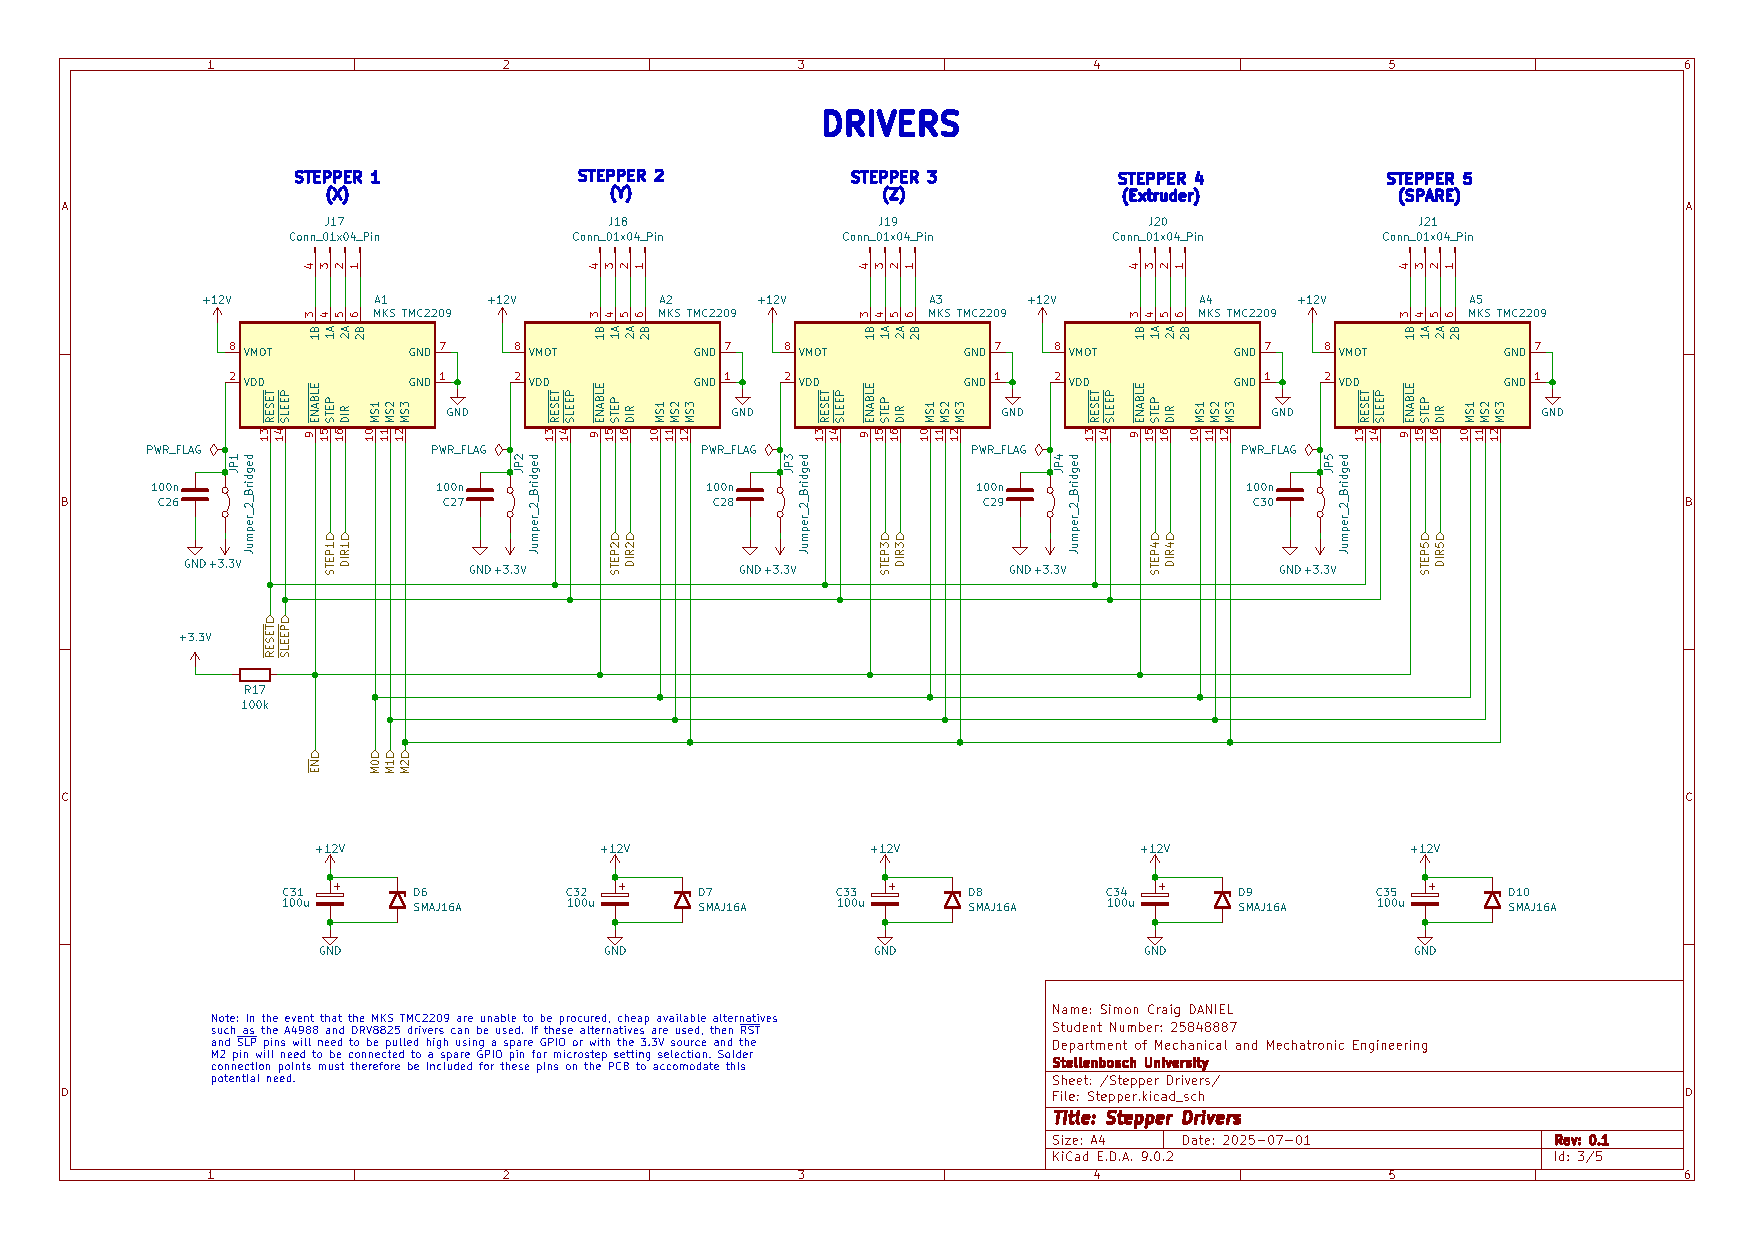
\includegraphics[angle=90, width=0.64\textheight]{chaps-append/PCBSchematic_Page3.pdf}
  \captionof{figure}{Bioprinter stepper driver system schematic.}
  \label{fig:pcb_steppers}

  \vspace{1em}
  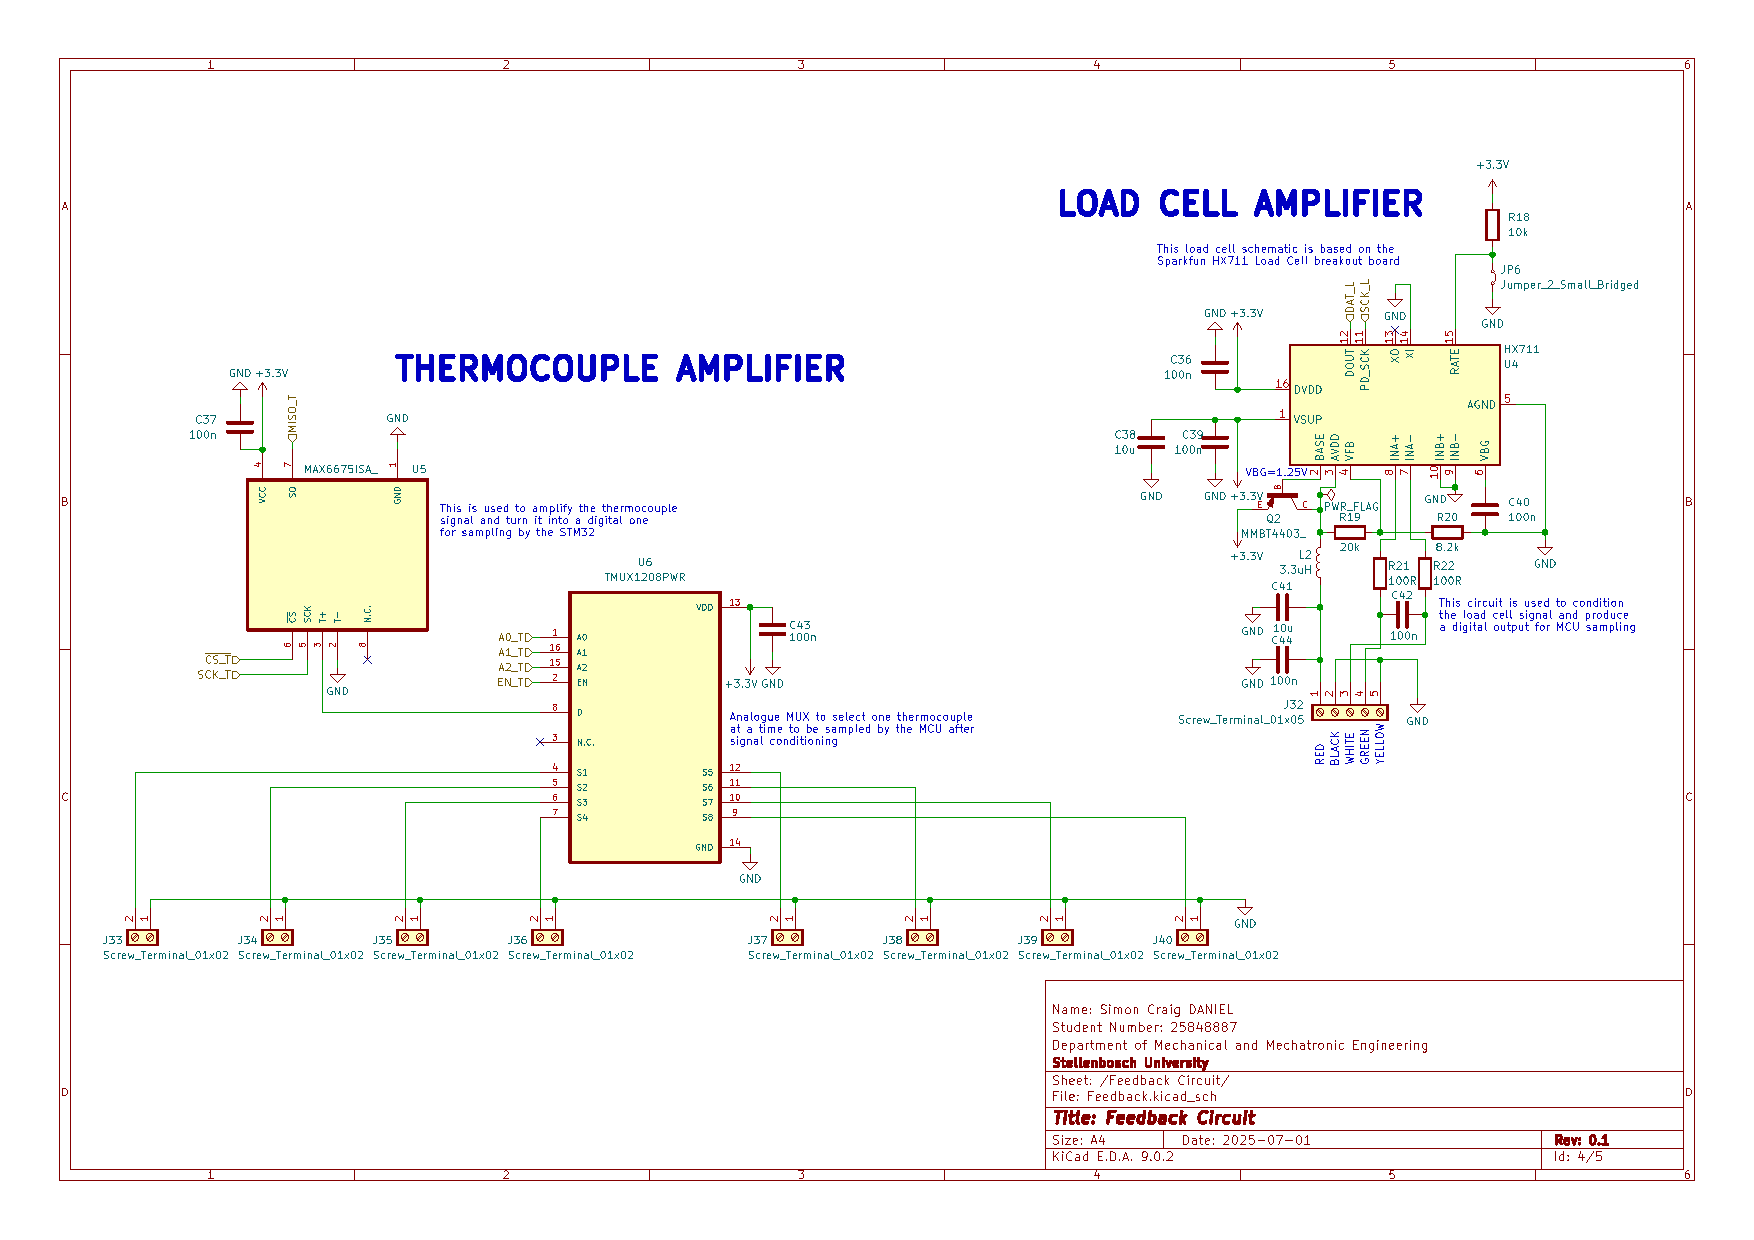
\includegraphics[angle=90, width=0.64\textheight]{chaps-append/PCBSchematic_Page4.pdf}
  \captionof{figure}{Bioprinter sensor system schematic.}
  \label{fig:pcb_sensors}

  \vspace{1em}
  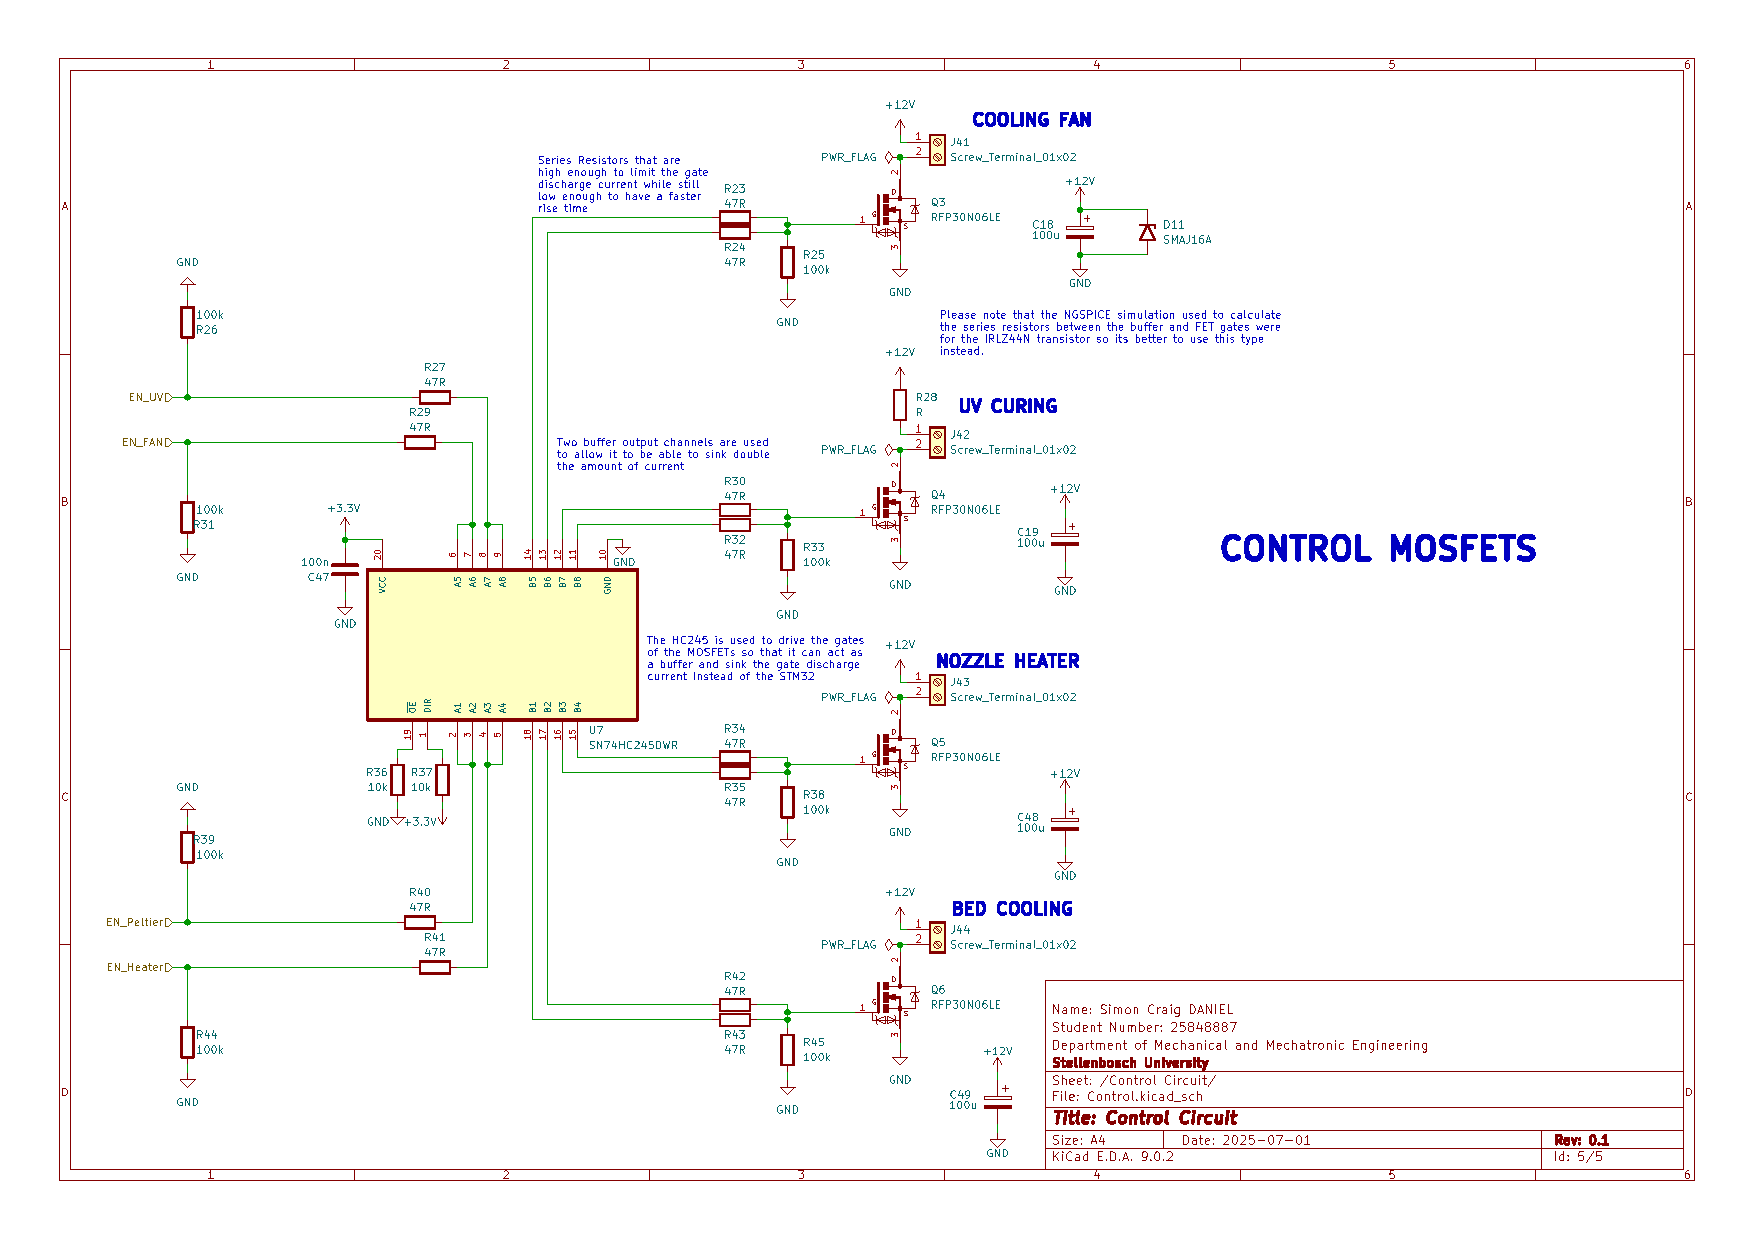
\includegraphics[angle=90, width=0.64\textheight]{chaps-append/PCBSchematic_Page5.pdf}
  \captionof{figure}{Bioprinter control circuit schematic.}
  \label{fig:pcb_control}
\end{center}
